% Options for packages loaded elsewhere
\PassOptionsToPackage{unicode}{hyperref}
\PassOptionsToPackage{hyphens}{url}
%
\documentclass[
]{book}
\usepackage{amsmath,amssymb}
\usepackage{lmodern}
\usepackage{ifxetex,ifluatex}
\ifnum 0\ifxetex 1\fi\ifluatex 1\fi=0 % if pdftex
  \usepackage[T1]{fontenc}
  \usepackage[utf8]{inputenc}
  \usepackage{textcomp} % provide euro and other symbols
\else % if luatex or xetex
  \usepackage{unicode-math}
  \defaultfontfeatures{Scale=MatchLowercase}
  \defaultfontfeatures[\rmfamily]{Ligatures=TeX,Scale=1}
\fi
% Use upquote if available, for straight quotes in verbatim environments
\IfFileExists{upquote.sty}{\usepackage{upquote}}{}
\IfFileExists{microtype.sty}{% use microtype if available
  \usepackage[]{microtype}
  \UseMicrotypeSet[protrusion]{basicmath} % disable protrusion for tt fonts
}{}
\makeatletter
\@ifundefined{KOMAClassName}{% if non-KOMA class
  \IfFileExists{parskip.sty}{%
    \usepackage{parskip}
  }{% else
    \setlength{\parindent}{0pt}
    \setlength{\parskip}{6pt plus 2pt minus 1pt}}
}{% if KOMA class
  \KOMAoptions{parskip=half}}
\makeatother
\usepackage{xcolor}
\IfFileExists{xurl.sty}{\usepackage{xurl}}{} % add URL line breaks if available
\IfFileExists{bookmark.sty}{\usepackage{bookmark}}{\usepackage{hyperref}}
\hypersetup{
  pdftitle={小蓝哥的知识荒原},
  pdfauthor={李详},
  hidelinks,
  pdfcreator={LaTeX via pandoc}}
\urlstyle{same} % disable monospaced font for URLs
\usepackage{color}
\usepackage{fancyvrb}
\newcommand{\VerbBar}{|}
\newcommand{\VERB}{\Verb[commandchars=\\\{\}]}
\DefineVerbatimEnvironment{Highlighting}{Verbatim}{commandchars=\\\{\}}
% Add ',fontsize=\small' for more characters per line
\usepackage{framed}
\definecolor{shadecolor}{RGB}{248,248,248}
\newenvironment{Shaded}{\begin{snugshade}}{\end{snugshade}}
\newcommand{\AlertTok}[1]{\textcolor[rgb]{0.94,0.16,0.16}{#1}}
\newcommand{\AnnotationTok}[1]{\textcolor[rgb]{0.56,0.35,0.01}{\textbf{\textit{#1}}}}
\newcommand{\AttributeTok}[1]{\textcolor[rgb]{0.77,0.63,0.00}{#1}}
\newcommand{\BaseNTok}[1]{\textcolor[rgb]{0.00,0.00,0.81}{#1}}
\newcommand{\BuiltInTok}[1]{#1}
\newcommand{\CharTok}[1]{\textcolor[rgb]{0.31,0.60,0.02}{#1}}
\newcommand{\CommentTok}[1]{\textcolor[rgb]{0.56,0.35,0.01}{\textit{#1}}}
\newcommand{\CommentVarTok}[1]{\textcolor[rgb]{0.56,0.35,0.01}{\textbf{\textit{#1}}}}
\newcommand{\ConstantTok}[1]{\textcolor[rgb]{0.00,0.00,0.00}{#1}}
\newcommand{\ControlFlowTok}[1]{\textcolor[rgb]{0.13,0.29,0.53}{\textbf{#1}}}
\newcommand{\DataTypeTok}[1]{\textcolor[rgb]{0.13,0.29,0.53}{#1}}
\newcommand{\DecValTok}[1]{\textcolor[rgb]{0.00,0.00,0.81}{#1}}
\newcommand{\DocumentationTok}[1]{\textcolor[rgb]{0.56,0.35,0.01}{\textbf{\textit{#1}}}}
\newcommand{\ErrorTok}[1]{\textcolor[rgb]{0.64,0.00,0.00}{\textbf{#1}}}
\newcommand{\ExtensionTok}[1]{#1}
\newcommand{\FloatTok}[1]{\textcolor[rgb]{0.00,0.00,0.81}{#1}}
\newcommand{\FunctionTok}[1]{\textcolor[rgb]{0.00,0.00,0.00}{#1}}
\newcommand{\ImportTok}[1]{#1}
\newcommand{\InformationTok}[1]{\textcolor[rgb]{0.56,0.35,0.01}{\textbf{\textit{#1}}}}
\newcommand{\KeywordTok}[1]{\textcolor[rgb]{0.13,0.29,0.53}{\textbf{#1}}}
\newcommand{\NormalTok}[1]{#1}
\newcommand{\OperatorTok}[1]{\textcolor[rgb]{0.81,0.36,0.00}{\textbf{#1}}}
\newcommand{\OtherTok}[1]{\textcolor[rgb]{0.56,0.35,0.01}{#1}}
\newcommand{\PreprocessorTok}[1]{\textcolor[rgb]{0.56,0.35,0.01}{\textit{#1}}}
\newcommand{\RegionMarkerTok}[1]{#1}
\newcommand{\SpecialCharTok}[1]{\textcolor[rgb]{0.00,0.00,0.00}{#1}}
\newcommand{\SpecialStringTok}[1]{\textcolor[rgb]{0.31,0.60,0.02}{#1}}
\newcommand{\StringTok}[1]{\textcolor[rgb]{0.31,0.60,0.02}{#1}}
\newcommand{\VariableTok}[1]{\textcolor[rgb]{0.00,0.00,0.00}{#1}}
\newcommand{\VerbatimStringTok}[1]{\textcolor[rgb]{0.31,0.60,0.02}{#1}}
\newcommand{\WarningTok}[1]{\textcolor[rgb]{0.56,0.35,0.01}{\textbf{\textit{#1}}}}
\usepackage{longtable,booktabs,array}
\usepackage{calc} % for calculating minipage widths
% Correct order of tables after \paragraph or \subparagraph
\usepackage{etoolbox}
\makeatletter
\patchcmd\longtable{\par}{\if@noskipsec\mbox{}\fi\par}{}{}
\makeatother
% Allow footnotes in longtable head/foot
\IfFileExists{footnotehyper.sty}{\usepackage{footnotehyper}}{\usepackage{footnote}}
\makesavenoteenv{longtable}
\usepackage{graphicx}
\makeatletter
\def\maxwidth{\ifdim\Gin@nat@width>\linewidth\linewidth\else\Gin@nat@width\fi}
\def\maxheight{\ifdim\Gin@nat@height>\textheight\textheight\else\Gin@nat@height\fi}
\makeatother
% Scale images if necessary, so that they will not overflow the page
% margins by default, and it is still possible to overwrite the defaults
% using explicit options in \includegraphics[width, height, ...]{}
\setkeys{Gin}{width=\maxwidth,height=\maxheight,keepaspectratio}
% Set default figure placement to htbp
\makeatletter
\def\fps@figure{htbp}
\makeatother
\setlength{\emergencystretch}{3em} % prevent overfull lines
\providecommand{\tightlist}{%
  \setlength{\itemsep}{0pt}\setlength{\parskip}{0pt}}
\setcounter{secnumdepth}{5}
\usepackage{ctex}

%\usepackage{xltxtra} % XeLaTeX的一些额外符号
% 设置中文字体
%\setCJKmainfont[BoldFont={黑体},ItalicFont={楷体}]{新宋体}

% 设置边距
\usepackage{geometry}
\geometry{%
  left=2.0cm, right=2.0cm, top=3.5cm, bottom=2.5cm} 

\usepackage{amsthm,mathrsfs}
\usepackage{booktabs}
\usepackage{longtable}
\makeatletter
\def\thm@space@setup{%
  \thm@preskip=8pt plus 2pt minus 4pt
  \thm@postskip=\thm@preskip
}
\makeatother
\ifluatex
  \usepackage{selnolig}  % disable illegal ligatures
\fi
\usepackage[style=apa,]{biblatex}
\addbibresource{mybib.bib}

\title{小蓝哥的知识荒原}
\author{李详}
\date{2021年10月13日}

\begin{document}
\maketitle

{
\setcounter{tocdepth}{1}
\tableofcontents
}
\hypertarget{ux7b80ux4ecb}{%
\chapter*{简介}\label{ux7b80ux4ecb}}
\addcontentsline{toc}{chapter}{简介}

我,李详,昵称小蓝哥。现于云南农业大学攻读植物病理学博士学位。

\hypertarget{r}{%
\chapter{R语言知识汇总}\label{r}}

\hypertarget{ux672cux7ae0ux524dux8a00}{%
\section{本章前言}\label{ux672cux7ae0ux524dux8a00}}

本章主要是关于R语言的相关知识,包括R语言基础知识、数据统计分析、数据可视化及机器学习等内容。

\hypertarget{python}{%
\chapter{Python知识汇总}\label{python}}

\hypertarget{ux672cux7ae0ux524dux8a00-1}{%
\section{本章前言}\label{ux672cux7ae0ux524dux8a00-1}}

本章主要是关于Python的相关知识,包括Python基础知识、数据统计分析、数据可视化及人工只能等内容。

\hypertarget{bioinf}{%
\chapter{生物信息学}\label{bioinf}}

\hypertarget{ux672cux7ae0ux524dux8a00-2}{%
\section{本章前言}\label{ux672cux7ae0ux524dux8a00-2}}

本章主要是关于生物信息学的相关知识。

\hypertarget{wslux5b89ux88c5ux4f7fux7528docker}{%
\section{\texorpdfstring{\texttt{WSL}安装使用\texttt{Docker}}{WSL安装使用Docker}}\label{wslux5b89ux88c5ux4f7fux7528docker}}

\hypertarget{dockerux7684ux5b89ux88c5}{%
\subsection{\texorpdfstring{\texttt{Docker}的安装}{Docker的安装}}\label{dockerux7684ux5b89ux88c5}}

参考的安装教程:\href{https://yeasy.gitbook.io/docker_practice/install/ubuntu}{Docker-从入门到实践}。关键的代码如下:

\begin{Shaded}
\begin{Highlighting}[]
\NormalTok{curl }\SpecialCharTok{{-}}\NormalTok{fsSL test.docker.com }\SpecialCharTok{{-}}\NormalTok{o get}\SpecialCharTok{{-}}\NormalTok{docker.sh}
\NormalTok{curl }\SpecialCharTok{{-}}\NormalTok{fsSL get.docker.com }\SpecialCharTok{{-}}\NormalTok{o get}\SpecialCharTok{{-}}\NormalTok{docker.sh}
\NormalTok{sudo sh get}\SpecialCharTok{{-}}\NormalTok{docker.sh }\SpecialCharTok{{-}{-}}\NormalTok{mirror Aliyun}
\NormalTok{sudo sh get}\SpecialCharTok{{-}}\NormalTok{docker.sh }\SpecialCharTok{{-}{-}}\NormalTok{mirror AzureChinaCloud}
\end{Highlighting}
\end{Shaded}

\hypertarget{dockerux7684ux4f7fux7528}{%
\subsection{\texorpdfstring{\texttt{Docker}的使用}{Docker的使用}}\label{dockerux7684ux4f7fux7528}}

\texttt{Docker}默认是需要\texttt{root}用户才能使用的,在\texttt{Windows上}我习惯于进入\texttt{Powershell}后执行下面的命令启动\texttt{Docker}:

\begin{verbatim}
wsl --shutdown # 先关闭wsl
wsl # 启动WSL
sudo su # 进入root
sudo service docker start # 启动Docker
su xiang # 切换会用户(非root权限)
\end{verbatim}

\hypertarget{ux5982ux4f55ux4ecewsl1ux5207ux6362ux5230wsl2}{%
\subsection{\texorpdfstring{如何从\texttt{WSL1}切换到\texttt{WSL2}}{如何从WSL1切换到WSL2}}\label{ux5982ux4f55ux4ecewsl1ux5207ux6362ux5230wsl2}}

我在\texttt{Windows}上使用\texttt{Docker}遇到的一个很奇怪的问题是,我之前的版本是\texttt{WSL1},\texttt{Docker}无论如何都无法使用,搜索半天也没有找到解决方法,索性将\texttt{WSL1}升级成\texttt{WSL2},没想到问题就那样解决了。参考教程:\href{https://zhuanlan.zhihu.com/p/356397851}{知乎:WSL1 升级为WSL2}。下面是升级的过程:

\begin{itemize}
\item
  下载对应的内核更新包:\href{https://link.zhihu.com/?target=https\%3A//wslstorestorage.blob.core.windows.net/wslblob/wsl_update_x64.msi}{点击下载}
\item
  \texttt{CMD}中管理员身份运行代码:

\begin{verbatim}
dism.exe /online /enable-feature /featurename:VirtualMachinePlatform /all /norestart
\end{verbatim}
\item
  设置版本

\begin{verbatim}
wsl --set-version Ubuntu-20.04 2
\end{verbatim}

  其中的\texttt{Ubuntu-20.04}是通过代码\texttt{wsl\ -l\ -v}查看到的。

  然后再次重启\texttt{WSL}即可。
\end{itemize}

\hypertarget{ux4e0bux8f7ddockerux955cux50cf}{%
\subsection{\texorpdfstring{下载\texttt{Docker}镜像}{下载Docker镜像}}\label{ux4e0bux8f7ddockerux955cux50cf}}

在\href{https://hub.docker.com/}{Docker Hub}中检索下载需要的镜像。

\hypertarget{dockerux7684ux4f7fux7528-1}{%
\subsection{\texorpdfstring{\texttt{Docker}的使用}{Docker的使用}}\label{dockerux7684ux4f7fux7528-1}}

进入\texttt{WSL}后运行下方代码运行\texttt{Docker}:

\begin{verbatim}
docker run -v /mnt/:/work -it omicsclass/rnaseq
\end{verbatim}

其中的\texttt{work}是不一定的,需要看镜像给的路径是啥。

\hypertarget{ux5982ux4f55ux521bux5efaux81eaux5df1ux7684ux955cux50cf}{%
\subsection{如何创建自己的镜像}\label{ux5982ux4f55ux521bux5efaux81eaux5df1ux7684ux955cux50cf}}

先从\href{https://hub.docker.com/}{Docker Hub}下载\texttt{Ubuntu}的官方镜像,然后在镜像中安装需要的软件。
PS:如何加速\texttt{pip}的下载:

\begin{verbatim}
pip install django -i https://pypi.tuna.tsinghua.edu.cn/simple
\end{verbatim}

加速的\texttt{R}包的下载安装:

\begin{Shaded}
\begin{Highlighting}[]
\FunctionTok{options}\NormalTok{(}\AttributeTok{repos=}\FunctionTok{structure}\NormalTok{(}\FunctionTok{c}\NormalTok{(}\AttributeTok{CRAN=}\StringTok{"https://mirrors.tuna.tsinghua.edu.cn/CRAN/"}\NormalTok{)))}
\FunctionTok{options}\NormalTok{(}\AttributeTok{BioC\_mirror=}\StringTok{"https://mirrors.tuna.tsinghua.edu.cn/bioconductor"}\NormalTok{)}
\end{Highlighting}
\end{Shaded}

\begin{figure}
\centering
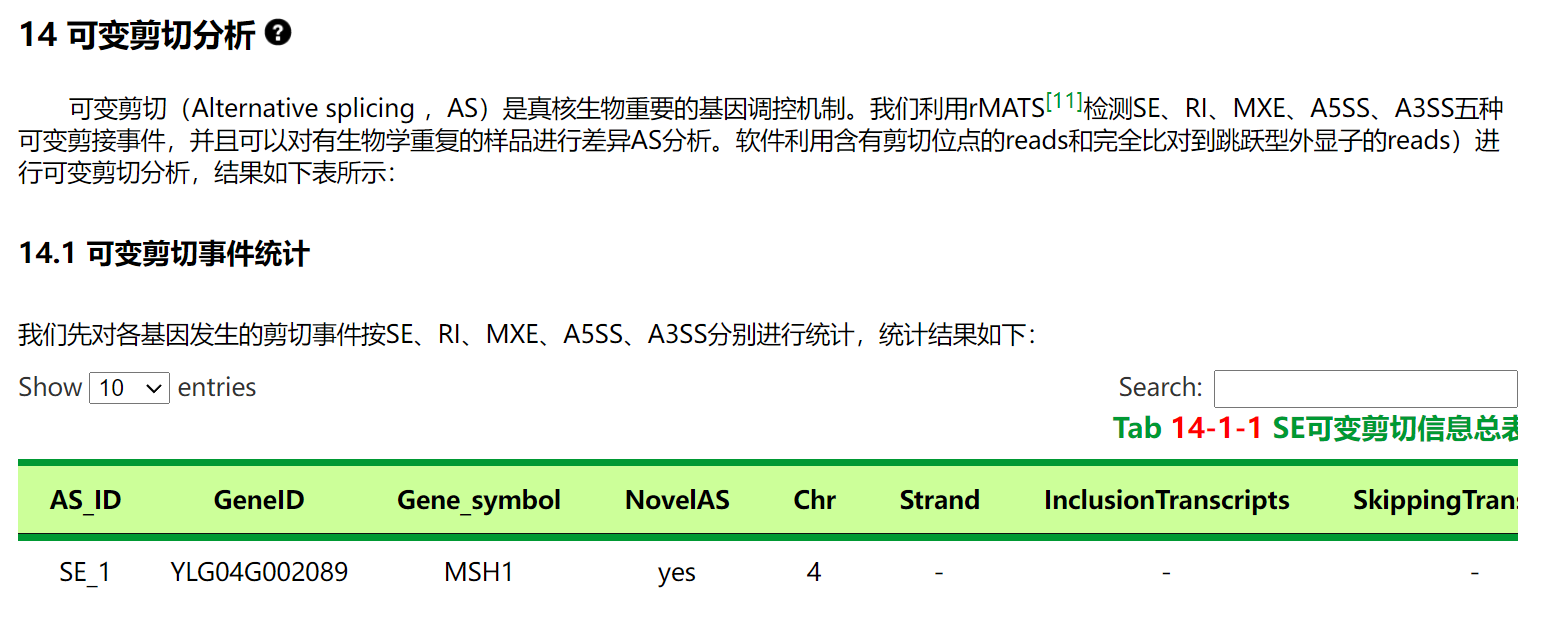
\includegraphics{figures/0.png}
\caption{123}
\end{figure}

\hypertarget{research}{%
\chapter{嗑盐过程的酸甜苦辣}\label{research}}

\hypertarget{ux672cux7ae0ux524dux8a00-3}{%
\section{本章前言}\label{ux672cux7ae0ux524dux8a00-3}}

本章主要与科研相关,包括但不限于文献阅读、科研绘图、实验方法等。

\hypertarget{other}{%
\chapter{Other}\label{other}}

\hypertarget{ux672cux7ae0ux524dux8a00-4}{%
\section{本章前言}\label{ux672cux7ae0ux524dux8a00-4}}

本章主要是关于软件安装使用等其他教程。

\printbibliography

\end{document}
